Abbiamo previsto tre layout differenti basati sulla dimensione dello schermo del device.
%\begin{figure}[h]
%        \centering
%        \begin{subfigure}[b]{0.10\textwidth}
%		
\includegraphics[scale=0.32]{images/articoli_desktop.png}
%		\caption{Screenshot desktop articoli.cgi}
%        \end{subfigure}
%        ~
%        \begin{subfigure}[b]{0.10\textwidth}
%		
\includegraphics[scale=0.30]{images/articoli_tablet.png}
%		\caption{Screenshot tablet articoli.cgi}
%        \end{subfigure}
%        ~
%        \begin{subfigure}[b]{0.30\textwidth}
%		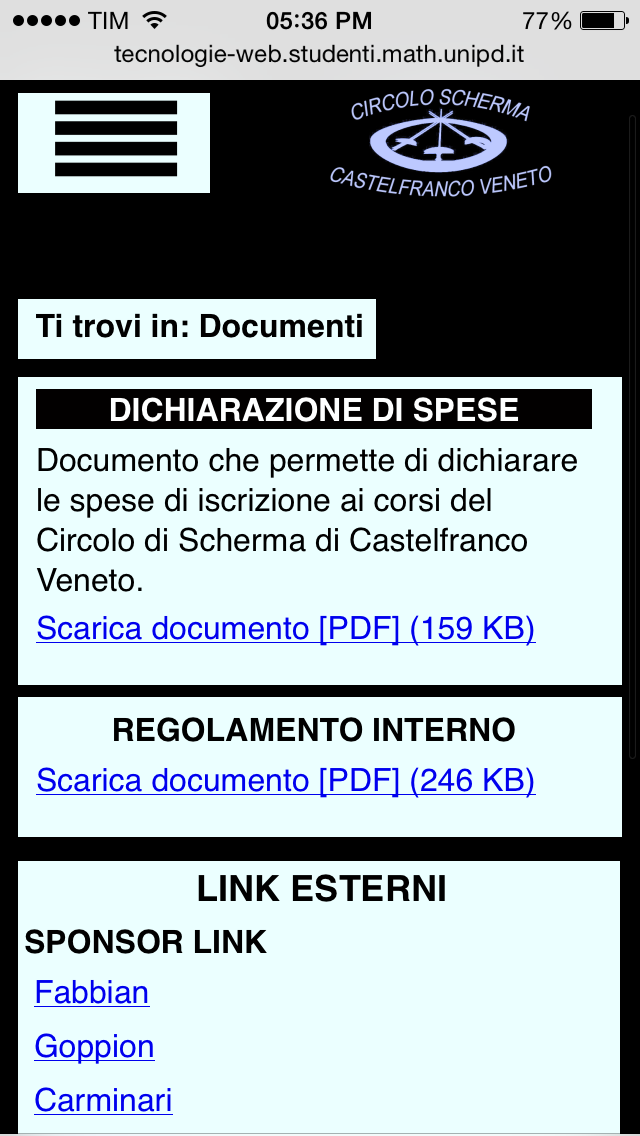
\includegraphics[scale=0.30]{images/articoli_mobile.png}
%		\caption{Screenshot mobile articoli.cgi}
%        \end{subfigure}
%        \caption{Layout schermi diversi}\label{layout}
%\end{figure}



Sono previste inoltre delle variazione del layout nel caso javascript sia disabilitato nel browser client. In particolare nelle pagine di inserimento o modifica della parte amministratore, vengono nascosti i bottoni dei tag speciali e la sidebar con la legenda, per far spazio ad una colonna con le istruzioni per inserire i tag correttamente.

%\begin{figure}[h!]
%        \centering
%        \begin{subfigure}[b]{0.48\textwidth}
%                \includegraphics[width=\textwidth]{images/formJavascript.png}
%                \caption{javaScript abilitato}
%                \label{javascript}
%        \end{subfigure}
%        ~
%        \begin{subfigure}[b]{0.48\textwidth}
%                \includegraphics[width=\textwidth]{images/formNoJavascript.png}
%                \caption{javaScript disabilitato}
%                \label{nojavascript}
%        \end{subfigure}
%        \caption{Layout con/senza javascript}\label{layoutJavascript}
%\end{figure}